\documentclass{article}
\usepackage[T1]{fontenc}
\usepackage{lmodern}
\usepackage{graphicx}
\usepackage{amsmath,amssymb}
\usepackage[a4paper,margin=2cm]{geometry}
\usepackage[absolute,overlay]{textpos}
\setlength{\TPHorizModule}{1mm}
\setlength{\TPVertModule}{1mm}
\usepackage[indonesian]{babel}
\usepackage{hyperref}
\setlength{\emergencystretch}{2em}
% unit: Halaman 68

\begin{document}

% === Halaman 68 (llm) ===

\begin{itemize}
  \item Post-quantum cryptography
\end{itemize}

\vspace{10mm}

\url{https://www.researchgate.net/figure/Basic-types-of-Post-Quantum-Cryptography-PQC_fig1_349071555}

% deskripsi: Diagram lingkaran yang menunjukkan empat tipe utama kriptografi pasca-kuantum (PQC): Hash-Based Signatures, Code-Based Cryptography, Multivariate Cryptography, dan Lattice-Based Cryptography.
% bbox normalisasi: [0.1530, 0.1820, 0.7600, 0.8340]
\begin{textblock*}{127.47mm}(32.13mm,54.05mm)
\noindent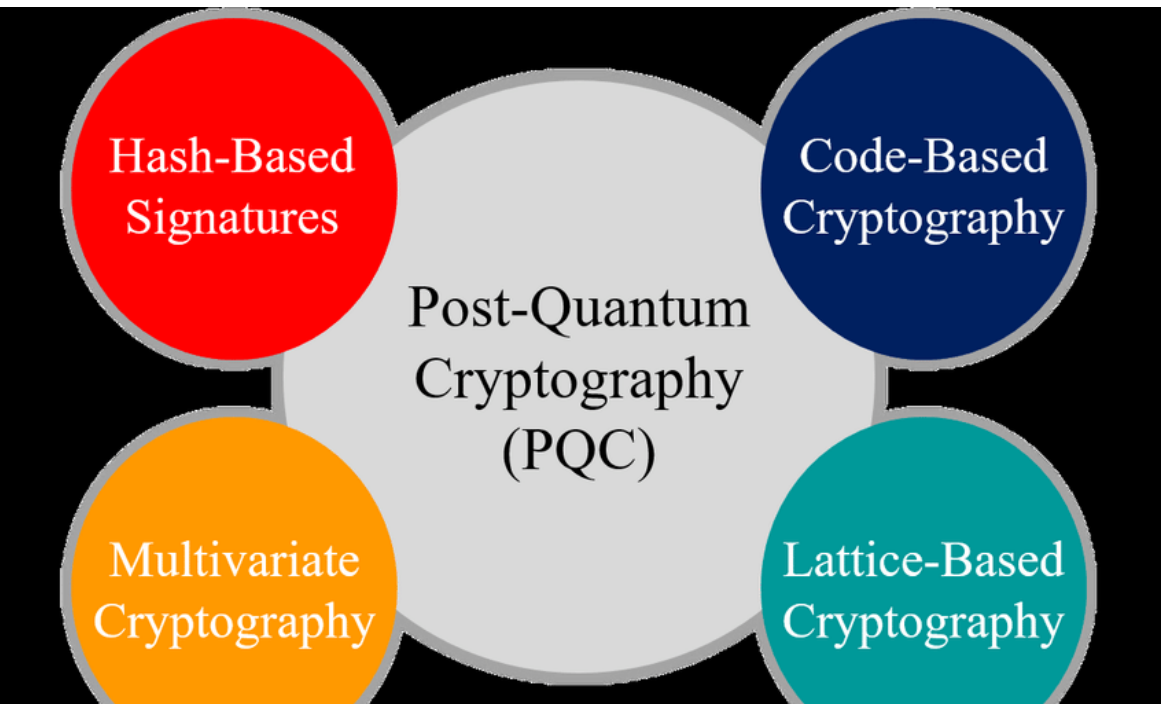
\includegraphics[width=127.47mm,height=193.64mm]{../../images/llm/page_068_img_01.png}%
\end{textblock*}

\end{document}
